%! Mode:: "TeX:UTF-8"
%! TEX program = xelatex
\PassOptionsToPackage{quiet}{xeCJK}
\documentclass[withoutpreface,bwprint]{cumcmthesis}
\usepackage{etoolbox}
\BeforeBeginEnvironment{tabular}{\zihao{-5}}
\usepackage[numbers,sort&compress]{natbib}  % 文献管理宏包
\usepackage[framemethod=TikZ]{mdframed}  % 框架宏包
\usepackage{url}  % 网页链接宏包
\usepackage{subcaption}  % 子图宏包
\newcolumntype{C}{>{\centering\arraybackslash}X}
\newcolumntype{R}{>{\raggedleft\arraybackslash}X}
\newcolumntype{L}{>{\raggedright\arraybackslash}X}


%%%%%%%%%%%%%%%%%%%%%%%%%%%%%%%%%%%%%%%%%%%%%%%%%%%%%%%%%%%%%
% 论文标题
\title{模拟含噪环境下的变分量子算法求解 $ \mathrm{H}_4 $ 分子基态能量}


%%%%%%%%%%%%%%%%%%%%%%%%%%%%%%%%%%%%%%%%%%%%%%%%%%%%%%%%%%%%%
%% 正文
\begin{document}

\maketitle
\begin{abstract}
在真实的量子计算机上,计算过程是通过重复的制备-采样过程来获得统计结果;且在当前中等规模含噪量子时代,硬件上存在不可忽视的噪声。
本赛题要求选手模拟量子真机的工作方式,在含噪条件下使用量子本征求解器求得 $ \mathrm{H}_4 $ 分子的基态能量,并提高解的精确度。
本文所提出的方案采用了基于硬件高效拟设的朴素量子本征求解器以最小化线路深度,对系统哈密顿量进行简化处理以降低噪声干扰。
此外,还基于预训练-微调的范式进行较为稳定的参数优化,并结合了读出误差缓解、零噪声外插值、参考态误差缓解等三种技术进行后处理降噪。
实验结果表明,所提方案平均分约为 244.76 分,最高分可达 3472.2812 分。

\keywords{含噪量子计算 \quad 量子误差缓解 \quad 量子本征求解器 \quad 分子基态能量}
\end{abstract}


%%%%%%%%%%%%%%%%%%%%%%%%%%%%%%%%%%%%%%%%%%%%%%%%%%%%%%%%%%%%%
% 目录
% \tableofcontents
% \newpage


%%%%%%%%%%%%%%%%%%%%%%%%%%%%%%%%%%%%%%%%%%%%%%%%%%%%%%%%%%%%%
\section{问题背景}

在中等规模含噪量子 (NISQ, noisy intermediate-scale quantum) 时代,量子计算机会受到各种内外噪声的影响而导致计算结果不精确,这对量子算法的设计而言是一个挑战。
而变分量子求解器 (VQE, variational quantum eigen-solver) 是一类有最可能在 NISQ 时代产生实际应用的变分量子算法,
其可用于物理系统的本征问题求解,如求解分子基态能量、线性方程组、组合优化等问题,因而受到广泛的关注。
分子基态能量求解是量子化学领域的一个基本问题,可使用变分量子求解器来实现计算加速。


%%%%%%%%%%%%%%%%%%%%%%%%%%%%%%%%%%%%%%%%%%%%%%%%%%%%%%%%%%%%%
\section{问题分析}

在量子化学领域,求解分子基态能量问题可参考如下流程:
首先获得分子的几何构型,如 $ \mathrm{H}_4 $ 分子由四个氢原子组成,取得每个原子的空间坐标、键长等信息;
然后借助玻恩-奧本海默近似、二次量子化、Hartree-Fock 方法和 Jordan-Wigner 变换,将分子信息分析并转换为 Pauli-哈密顿量矩阵的形式,
此矩阵的各特征值和特征向量即描述了该分子系统的离散能级和能量情况,从而将物理化学上的能量问题转换为数学上的矩阵本征问题;
最后依据公式 \ref{eq:rr-method} 所示的 Rayleigh–Ritz 不等式,构造变分量子线路 $ U(\theta) $ 以制备试探波函数 $ \Psi $,
通过不断优化参数 $ \theta $ 以最小化不等式右端,即可逼近左端的理论基态能量 $ E_0 $,此时的态矢 $ \left| \Psi \right> $ 也将逼近基态。

\begin{equation}
E_0 \le \frac{\left< \Psi  \right| \hat H \left| \Psi \right>}{\left< \Psi | \Psi \right>} = \left< U(\theta)  \right| \hat H \left| U(\theta) \right>
\label{eq:rr-method}
\end{equation}


%%%%%%%%%%%%%%%%%%%%%%%%%%%%%%%%%%%%%%%%%%%%%%%%%%%%%%%%%%%%%
\section{解决方案}

我们的解决方案主要包含四部分:哈密顿量近似简化、拟设选择、基于预训练-微调的参数优化、误差缓解后处理。

\subsection{哈密顿量近似简化}

哈密顿量简化包含两个步骤:X-Y近似,舍去小系数项。
首先,我们观察到在理想无噪环境下,系统的哈密顿量 $ \hat H $ 具有比较显著的对称性。
具体而言,哈密顿量可被分解为一系列 Pauli串 (一组Pauli算符的张量积) 的线性加权和,即 $ \hat H = \sum_k \alpha_k * s_k $。
在此分解中可观察到大量成对而系数 $ \alpha_k $ 相同的Pauli串,在字母上仅有 X 和 Y 相互替换的差别。
测试可发现,这样成对的两个串的哈密顿量期望值是一样的,因此我们可以合并它们,极大减少了需要测量的 Pauli 串数量。
然后,近似合并后的 Pauli 串中有大量系数很小的项,考虑到它们对结果数值的贡献较小,我们将忽略绝对值小于 1e-2 的项。
综合两步操作,Pauli串数量从 184 减少至 66,降低了 64.13\% 。

\subsection{拟设选择}

变分本征求解器中的拟设 (Ansatz) 线路通常有两种设计思路,其一是受物理原理启发,其二是受软硬件架构约束。
在第一类方法中,基于耦合簇方法的 UCC \cite{UCC2017} 系列拟设在模拟器上可取得十分精确的结果,但因其线路过长而无法在当前含噪中等规模量子计算机上运行。
后续一系列简化改进的尝试,诸如化学紧凑启发式拟设 CHC \cite{CHC2020} 等,虽然已经在数量级意义上降低了线路长度,但当前真机条件依旧无法处理。
而在第二类方法中,硬件高效拟设 HEA \cite{HEA2017} 在设计上有较高自由度,故成为一个常见的选择。

我们设计的 HEA 具体线路结构如图 \ref{fig:ansatz} 所示,使用 8 个量子比特、57 个门、32 个可学习参数。
重复多轮优化,并在每轮优化收敛后进行线路剪枝,剪枝策略为移除旋转角绝对值小于阈值 1e-5 的旋转门,最终在多次优化-剪枝后仅需约 35 个门、10 个参数。
注意到线路最末端的四个 X 门实际组成了 HF 态线路,这将用于后续的参考态误差缓解。
优化后的含参线路在理想无噪环境下的哈密顿期望值为 -2.138179955146652,相对真实值 -2.1663874486347643 而言的误差为 1.30\%。

\begin{figure}
	\centering
	\subcaptionbox{初始拟设线路}
	{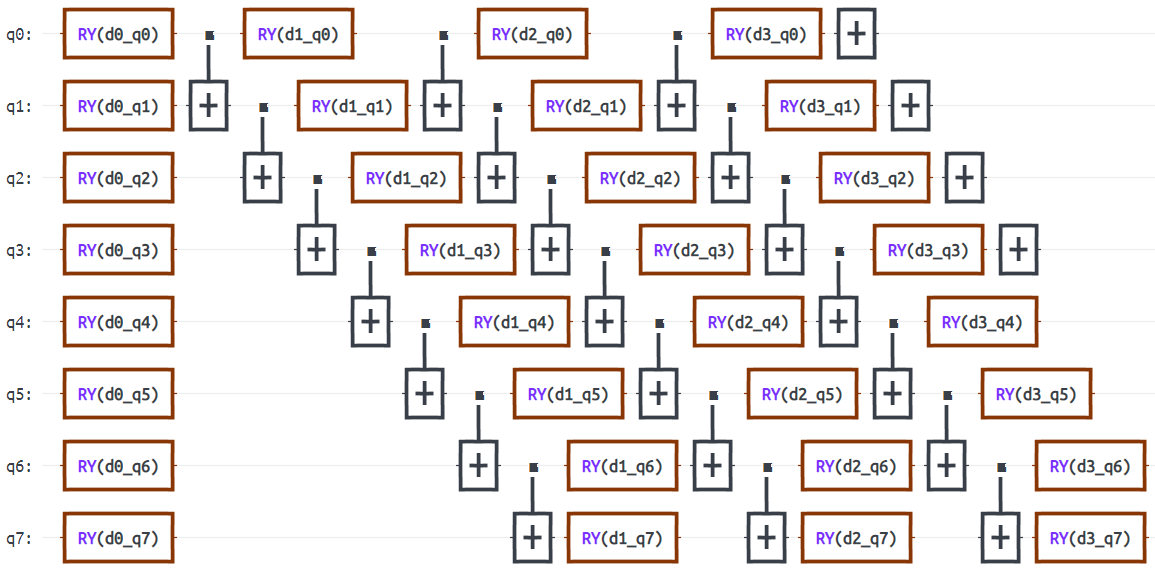
\includegraphics[width=0.48\textwidth]{figures/ansatz-before.png}}
	\subcaptionbox{优化-剪枝后拟设线路}
	{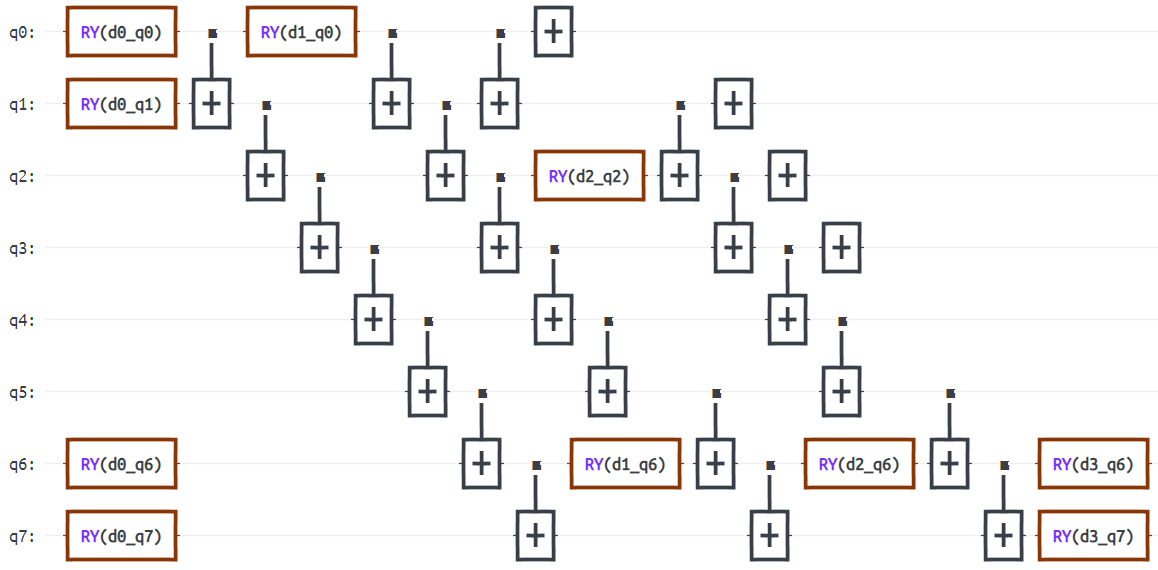
\includegraphics[width=0.48\textwidth]{figures/ansatz-after.png}}
	\caption{拟设线路设计}
	\label{fig:ansatz}
\end{figure}

\subsection{基于预训练-微调的参数优化}

注意到构型大致相似的 $ \mathrm{H}_4 $ 分子体现在波函数上只有振幅上的微小差异,因此我们可以考虑使用预训练-微调的范式来优化变分线路,即从一个已知的次优解出发,而非总是从随机或全零初始化出发去寻找更优解,从而加快收敛速度。
我们以单位键长、链状排布的 $ \mathrm{H}_4 $ 分子为基准,使用 Basin Hopping 算法进行全局优化搜索,寻找对应哈密顿量在给定 ansatz 的最优解 $ \theta^\ast $。
此后,对于其他几何构型的情况,再基于上述预训练 $ \theta^\ast $ 使用 Adam、COLBYLA 等方法进行局部优化。

\subsection{误差缓解后处理}

我们将结合读出误差缓解 (REM, Readout-error mitigation) \cite{REM2021} 、零噪声外插值 (ZNE, zero noise extrapolation) \cite{ZNE2017} 、参考态误差缓解 (RSEM, reference-state error mitigation) \cite{RSEM2022} 这三种技术来进行误差缓解后处理。

针对赛题给定的噪声模型,我们使用单个 RY 门做了基准测试,即使用连续 k 个门来累计旋转角度 $ 2 \pi $,并在计算基上测量 $ \left| 0 \right> $ 态的概率,实验结果如图 \ref{fig:noise} 所示。
可见随着横轴 RY 门的数量 $ k $ 增大,投影概率 (黄) 呈明显的线性下降趋势,而方差 (蓝) 则基本维持在一个水平线上下波动不大。
这个观察首先暗示了 ZNE 应当是可行的;其次,即使 $ k $ 很小的时候,投影概率也只有约 0.9,这意味着读出误差接近 10\%,需要进行 REM。

\begin{figure}
	\centering
	\subcaptionbox{RY门噪声基准测试\label{fig:noise}}
	{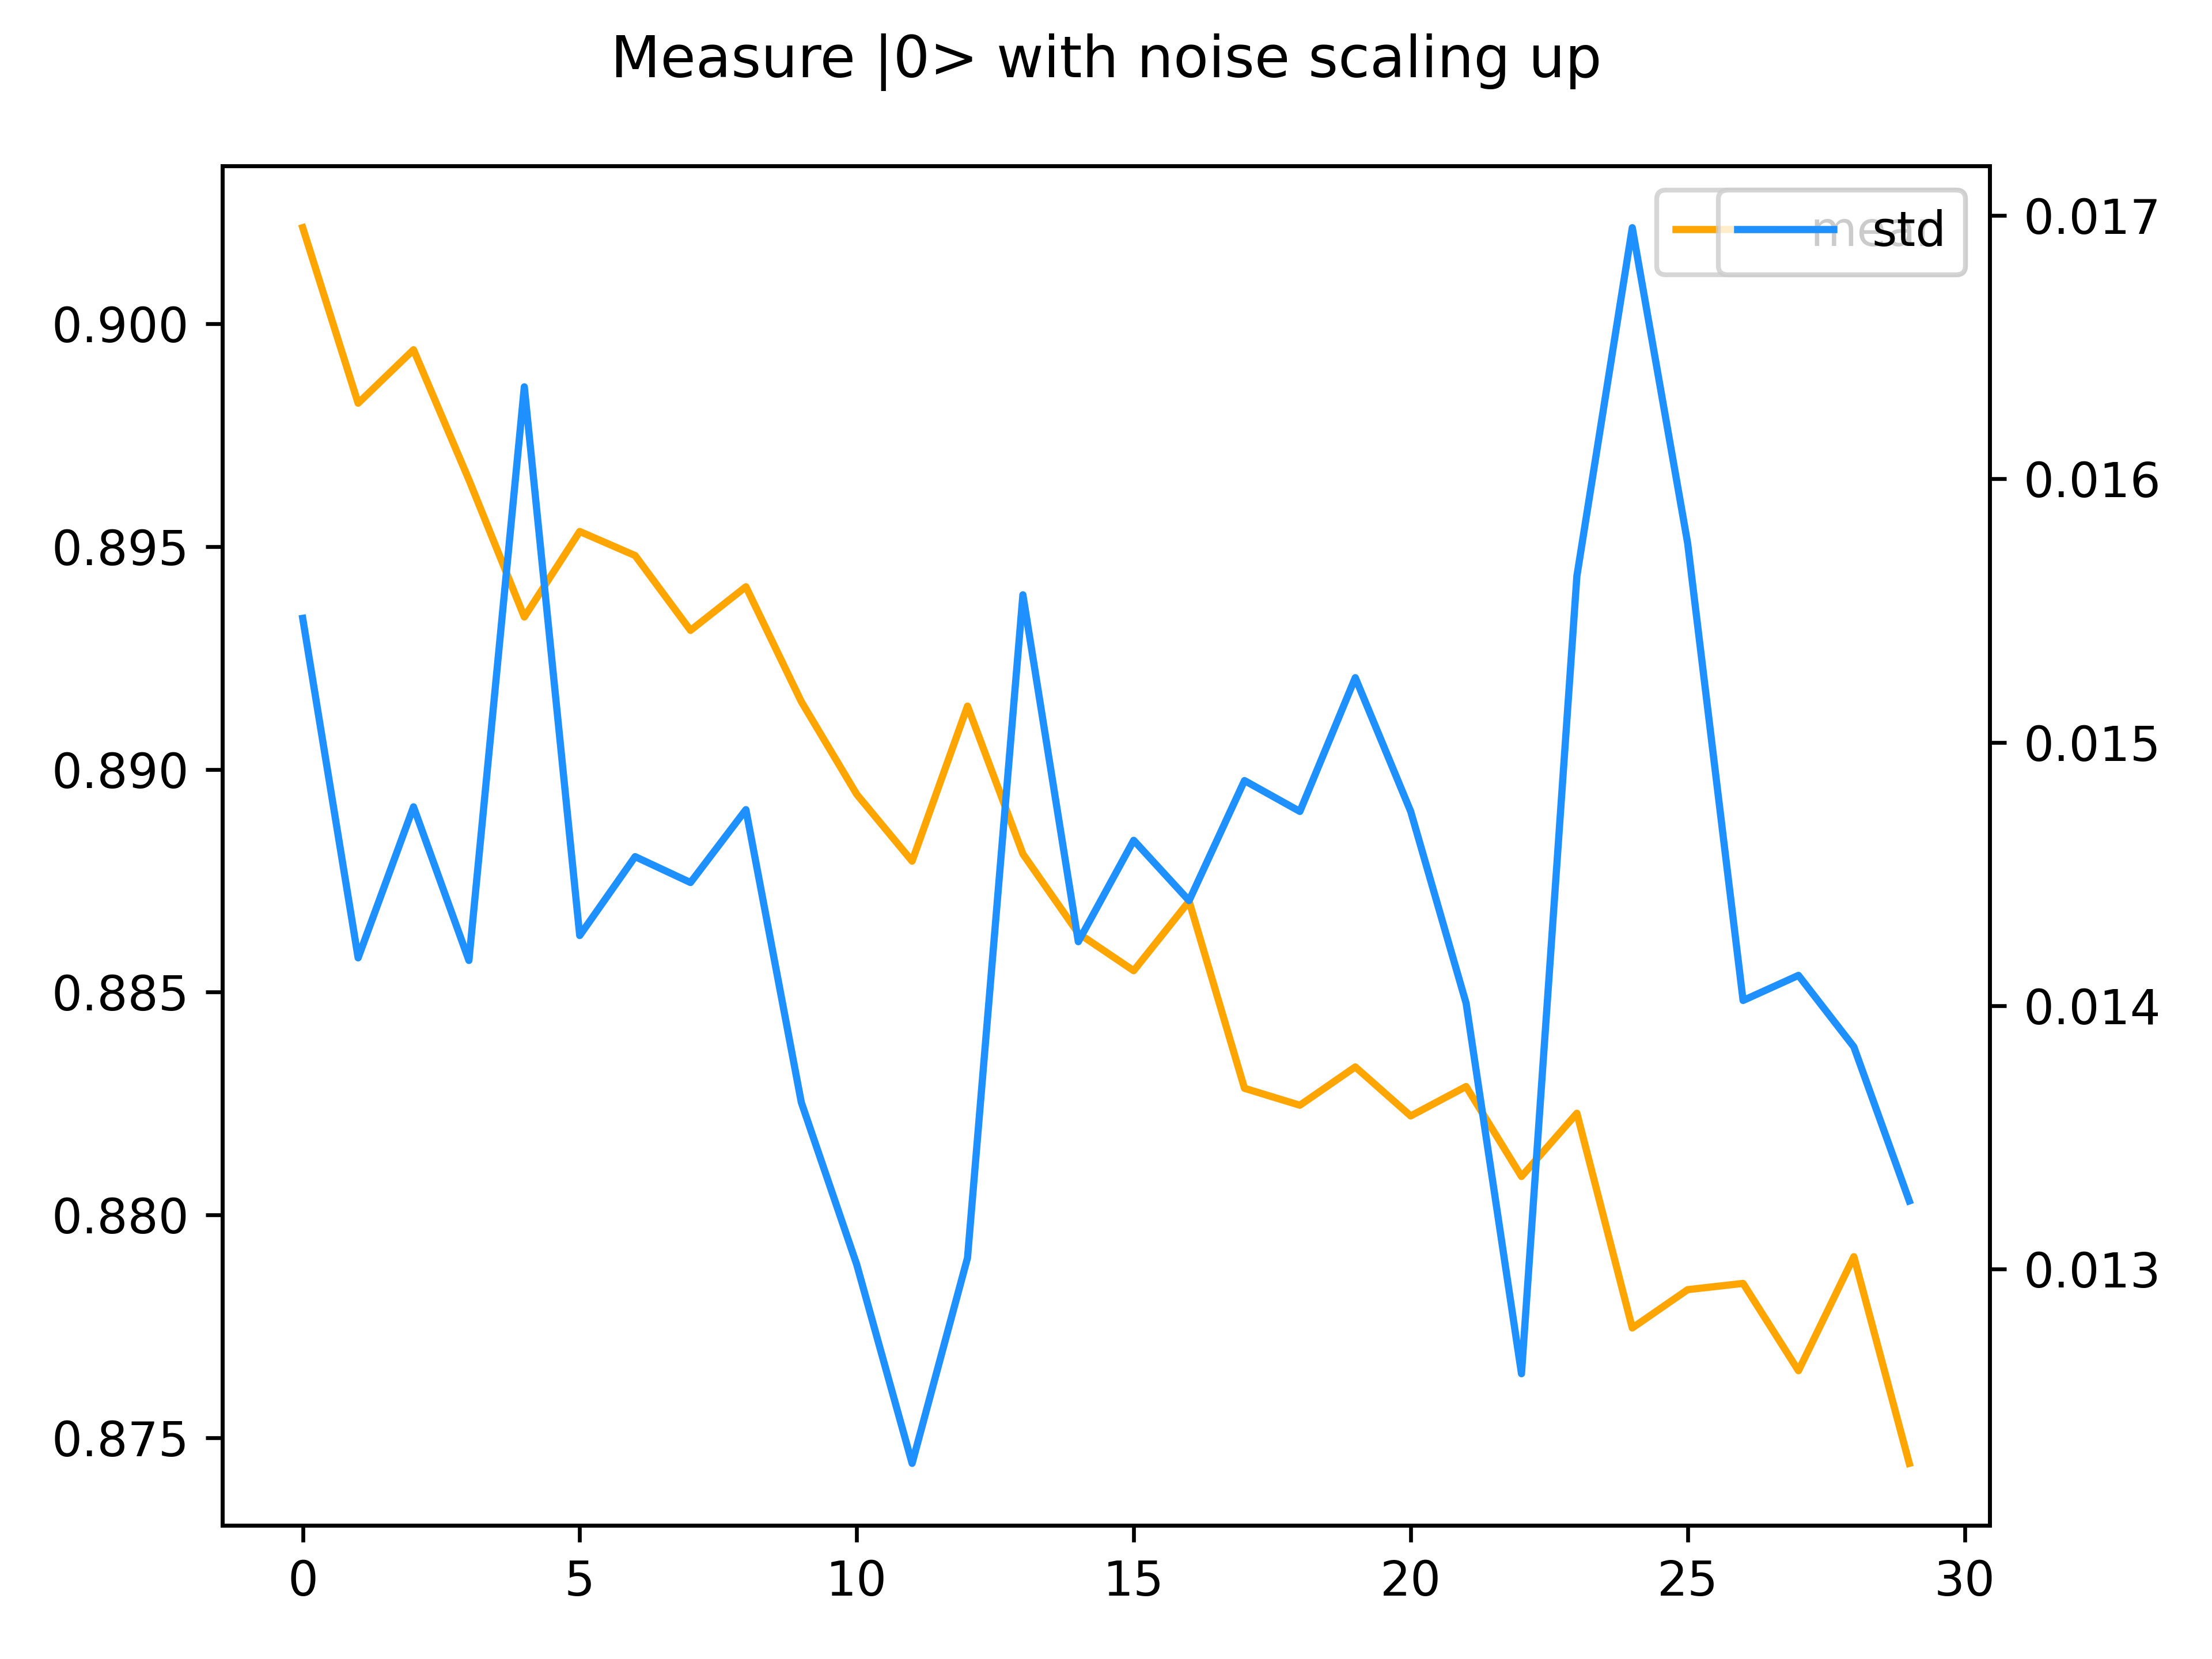
\includegraphics[width=0.48\textwidth]{figures/vis_noise_scale.png}}
	\subcaptionbox{参考态误差缓解\label{fig:RSEM}}
	{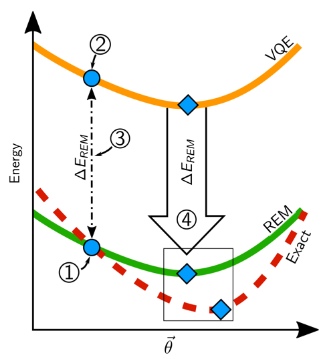
\includegraphics[width=0.48\textwidth]{figures/RSEM.png}}
	\caption{噪声测定与误差缓解}
\end{figure}

首先进行 REM,一般做法是进行一系列基准测量获得一个矫正表矩阵 (calibration table),其类似于一个二分类混淆矩阵,将测量结果乘上此矩阵的逆,或者进行最小二乘法拟合即可获得校正后的值。
但考虑到赛题中是一个人工模拟的噪声模型,即各量子比特表现同质化,故对于 REM 的实现可以直接退化为线性放缩,放缩因子可近似取 \ref{fig:noise} 中测定的黄线在 $ k = 1 $ 时的情况。
其次进行 ZNE,根据其原理将线路中的门扩展为 3、5、7 倍,即对每个门均追加一对同类但关系互逆的门,以此来放大噪声,并向左外插值出 0 倍噪声时的情况。
最后,我们尝试了比 ZNE 更轻量化的 RSEM,其基本原理如图 \ref{fig:RSEM} 所示:若假设线路的噪声情况不会依赖于参数 $ \theta $ 的取值,即红色虚线可以近似为绿色实线,则变分线路测定值 (黄) 可认为与校正值 (绿) 仅相差一个固定常数偏移;
通过巧妙的线路设计,我们可以先验得知这个常数,从而将测定值 (黄) 偏移为 矫正值 (绿),在近似意义上逼近真值 (红)。
实验结果表明,RSEM 不仅额外开销远小于 ZNE,并且准确度也更高,这可能是给定的噪声模型并不太符合线性扩展规律导致的,从而使得多次估值的 ZNE 会有更多的累计误差。


%%%%%%%%%%%%%%%%%%%%%%%%%%%%%%%%%%%%%%%%%%%%%%%%%%%%%%%%%%%%%
\section{结果}

\begin{table}[h!]
	\centering
	\caption{实验结果}
	\begin{tabular}{lll}
		\textbf{本地分数↑} & \textbf{提交分数↑} & \textbf{说明} \\
		\hline
		1.035 & \underline{0.5226} & baseline, trim coeff=1e-3, shot=30 \\
		1.334 & 0.574  & HEA(RY), trim coeff=1e-3, shots=100 \\
		2.360 & 1.0077 & HF, trim coeff=1e-3, shots=100 \\
		3.908 & 3.826  & HEA(RY), trim coeff=1e-3, shots=100, n\_meas=10 \\
		4.519 & 4.2442 & HEA(RY)\_no\_HF, trim coeff=1e-3, shots=100, n\_meas=10 \\
		6 $ \sim $ 63 & 27.9413 & HF, Z\_only, shots=10, n\_meas=10 \\
		14.740 & \textbf{15.4219} & HF, Z\_only (+exp\_fix), shots=100 (exactly $E_{HF}$) \\
		15.317 & 17.0523 & HEA(RY), depth=3, shots=100 \\
		 8.426 & 13.4319 & HEA(RY), depth=3, shots=500 \\
		17.266 & 19.3466 & HEA(RY), depth=3, shots=1000 \\
		16.958 & 18.6189 & HEA(RY), depth=3, shots=3000 \\
		7.924 $ \sim $ 87.44 & 9.6134 $ \sim $ 25.224 & HEA(RY, 3), init=randn, optim=Adam, shots=1000 \\
		9 $ \sim $ 33 & 15.9935 $ \sim $ 47.1661 & HEA(RY, 3), init=randn, optim=Adam, shots=10000, combine\_XY, rescaler \\
		8.038 $ \sim $ 26.389 & 32.0759 $ \sim $ 127.9223 & HEA(RY, 2), init=randn, optim=Adam, shots=1000, combine\_XY, rescaler \\
		203.663 & \textbf{12.5186 $ \sim $ 3472.2812} & HEA(RY, 3), init=pretrained, optim=Adam(lr=1e-4), shots=1000, combine\_XY, rescaler \\
	\end{tabular}
	\label{tbl:result}
\end{table}

我们的一系列实验结果如表 \ref{tbl:result} 所示,具体超参数配置比较繁琐按下不表,主要看\textbf{最后一行}即我们融合了所有有效技术的最终提交配置。
量子计算具有其内在的随机性,即使我们已经尽力降低这种随机性了,结果的方差仍然较大。
最低得分 12.5186 大约在 $ 10^1 $ 分的量级,而最高分 3472.2812 则达到了 $ 10^3 $ 分的量级,平均值落在 $ 10^2 $ 量级,经 28 次实验平均统计约 244.76 分。
经过排查我们初步发现,主要原因在于 openfermion 库在从分子构型分析哈密顿量这一步的算法是非确定性的,并且浮点计算中出现了负数的 0(暂时不知道是否为bug)。
这使得两个数值上完全相等的哈密顿量所变分优化出来的基态态矢的保真度不高,进一步导致基于预训练-微调的参数优化方式在一次实验中可能表现结果极端的好或者极端的坏。

【注】关于我们最高分 3472.2812 的讨论:
在我们连续两个月的屡次实验中,碰巧发现过在所用的三层 HEA(RY) 线路结构中存在一套特定参数,会使得变分线路的哈密顿量期望值达到 -2.1662148963146652,非常接近理论值!
但这一套参数非常难以搜索到,由于当时代码不完善,实验在半夜进行、无人值守,日志记录仅保存了末态态矢,及其与真值的保真度,并未记录这一套参数取值。
而后来多次的线上提交中我们刷出来这个异常高分,回想起之前的实验,我们猜想很可能就是优化器撞运气又重新找到了这组参数……


%%%%%%%%%%%%%%%%%%%%%%%%%%%%%%%%%%%%%%%%%%%%%%%%%%%%%%%%%%%%%
\section{总结及展望}

本文探索了含噪环境下模拟量子真机运行量子本征求解器以求解 $ \mathrm{H}_4 $ 分子基态能量,
综合应用了哈密顿量近似简化、硬件高效拟设设计、基于预训练-微调的参数优化、误差缓解后处理等技术和技巧,获得了较好的结果。
但解决量子噪声、量子测量随机性对结果的干扰仍然任重道远。


%%%%%%%%%%%%%%%%%%%%%%%%%%%%%%%%%%%%%%%%%%%%%%%%%%%%%%%%%%%%%
%% 参考文献
\newpage
\nocite{*}
\bibliographystyle{gbt7714-numerical}  % 引用格式
\bibliography{ref.bib}  % bib源


%%%%%%%%%%%%%%%%%%%%%%%%%%%%%%%%%%%%%%%%%%%%%%%%%%%%%%%%%%%%%
%% 附录
\newpage
\begin{appendices}

\section{主要代码}

哈密顿量近似简化:

\lstinputlisting[language=python]{code/ham_approx.py}

\end{appendices}
\end{document}